


\subsection{muP parametrization}

It is natural to ask if muP allows hyperparameter transfer across token horizons. To investigate this we consider the 50m model from \Cref{table:param}, and use muP parameterization. Note, we will not perform hyperparameter transfer across model sizes, we just use the muP parameterization which slightly differs from the standard parameterization of transformers. We then run ablation experiments using token horizons $\{25, 50, 100\}$ billion tokens and LRs of $\{0.25, 0.5, 1, 2, 4\}$ times the base LR in \Cref{table:param}. The results of this experiment are shown in \Cref{fig:mup}, and we can indeed see that the optimal LR decreases with a longer token horizon. We thus conclude that \textbf{the optimal LR does not transfer across token horizons with muP}.

\begin{figure}[]
\begin{center}
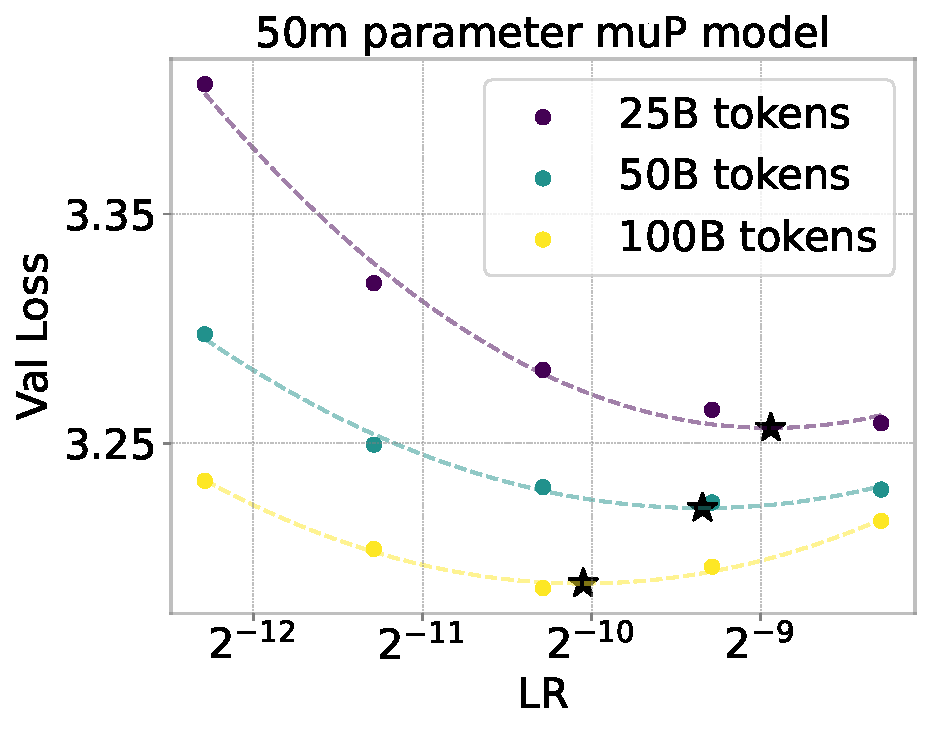
\includegraphics[width=0.55\textwidth]{images/mup.pdf}
\vspace{-0.3cm}
\caption{Optimal LR vs token horizon for a 50m model using muP parameterization \citep{mup}. We see that the optimal LR decreases with longer token horizons, demonstrating that LR does not transfer across horizons even with muP.}
\label{fig:mup}
\centering
\end{center}
\end{figure}



\subsection{Quantifying Variance}


\label{sec:uncertainty}

To ensure that our results are reliable we here consider quantifying the variance of our experiments. We will use two different methodologies. Firstly we use bootstrapping, following \cite{hoffmann2022training}. We consider the 350m model of \Cref{table:param}, randomly remove 20\% of the data points, and then fit the optimal LR at each token horizon and the scaling law of \Cref{eq:powerlaw}. We repeat this procedure 1000 times and then measure the mean and std of the optimal LR and the constants of \Cref{eq:powerlaw}. The results are given in \Cref{table:bootstrap_stds}. We see that the standard deviations are relatively small, which again suggests that the variance in our experimental results is low.


The second methodology we use is simply rerunning a small-scale experiment with multiple seeds. We use the 350m model from \Cref{table:param}, a 100B token horizon, three learning rates, and two additional seeds. We then estimate the optimal LR via a quadratic fit as in \Cref{sec:initial_abl}. The results of this experiment are shown in \Cref{table:seed_stds} in \Cref{appendix:experimental_data}. We see that there are small differences in the losses, and hence small differences in the estimated optimal LR. The relative std $\sigma/\mu$ is \scinot{2.63}{-2}, so we can expect the relative error to be a few percent. When using more data points the variance could further decrease due to concentration of measure.










\begin{table}[]
    \begin{center}
\begin{tabular}{llllll}
\toprule
&  25B &              50B &             100B &             200B &             400.0 \\
\midrule
$\mu(LR^*)$ &\scinot{7.04}{-4} & \scinot{5.96}{-4} & \scinot{5.07}{-4} & \scinot{3.45}{-4} & \scinot{2.44}{-4} \\
$\sigma(LR^*)$ &\scinot{1.28}{-5} & \scinot{9.12}{-6} & \scinot{1.96}{-5} & \scinot{4.07}{-6} & \scinot{4.31}{-6} \\
$\sigma/\mu$ &\scinot{1.82}{-2} & \scinot{1.53}{-2} & \scinot{3.88}{-2} & \scinot{1.18}{-2} & \scinot{1.76}{-2} \\
\bottomrule
\end{tabular}
\end{center}
\caption{We estimate the mean $\mu$ and standard deviation $\sigma$ of the optimal learning rate $\optlr$ via bootstrapping. We sample 80\% of the data from \Cref{fig:350m_curves} and then estimate the optimal LR with the procedure from \Cref{sec:initial_abl}. This bootstrapping procedure is repeated 1000 times. We see that the variance is small compared to the mean, and the relative error $\sigma/\mu$ is on the order of a few percent. This implies that the uncertainty in our estimates is small.}
\vspace{-0.3cm}
\label{table:bootstrap_stds}
\end{table}




\subsection{Effect of Batch Size}\label{sec:bs}

It is well known that batch size $BS$ affects the optimal LR \citep{imagenet1h}. While we primarily focus on the setting of a fixed batch size, we here consider modifying the batch size for the 1.3B model of \Cref{table:param}. Specifically, we double the batch size to 1m tokens and train for 25B and 50B tokens in total with different LRs. In \Cref{fig:curves_bs} in the Appendix we show the final validation loss as a function of the LR and estimate the optimal LR. In \Cref{fig:bs_main} we show the optimal LR as a function of token horizon for the 1.3B model using a batch size of 0.5 or 1m tokens. We see that the optimal LR is higher with a larger batch size as expected. More importantly, we note that the linear fits are roughly parallel. This suggests that the optimal LR depends on the token horizon the same way irrespective of the batch size, i.e. that we can factorize \Cref{eq:powerlaw} as $LR(BS, D) = f(BS) D^{-\beta}$.

